\documentclass[a4paper,10pt]{article}
\usepackage{graphicx}
\usepackage{lscape}
\usepackage{makecell}
\title{Results}
\author{}
\date{\today}
\begin{document}
\maketitle




\section{Tables of Friedman, Iman-Davendport, Holm-Hochberg and Nemenyi}
\begin{table}[!htp]
\centering
\caption{Comparison and Ranking od METRIC across classifiers}
\resizebox{\textwidth}{!}{%
\begin{tabular}{rllllllll}
Dataset&KNN8&Tree&MLP10&RF&SVM&Bayes&GBC&Ada\\
\Xhline{2\arrayrulewidth}
art\_rt&0.666 (6)&0.580 (8)&0.692 (5)&0.664 (7)&0.760 (2)&0.694 (4)&0.752 (3)&0.784 (1)\\
art\_w\_atleta&0.646 (5)&0.570 (7)&0.744 (1)&0.542 (8)&0.684 (3)&0.638 (6)&0.676 (4)&0.732 (2)\\
art\_w\_braso&0.590 (4)&0.540 (7)&0.572 (5)&0.508 (8)&0.676 (2)&0.692 (1)&0.636 (3)&0.544 (6)\\
art\_w\_campana&0.638 (6.5)&0.520 (8)&0.652 (5)&0.638 (6.5)&0.700 (2)&0.678 (3)&0.668 (4)&0.708 (1)\\
art\_w\_gato&0.706 (1)&0.550 (8)&0.636 (5)&0.626 (7)&0.676 (3)&0.672 (4)&0.684 (2)&0.632 (6)\\
art\_w\_petaka&0.594 (7)&0.570 (8)&0.668 (5)&0.674 (4)&0.708 (3)&0.716 (2)&0.724 (1)&0.616 (6)\\
fon\_rt&0.522 (6)&0.540 (5)&0.516 (7)&0.616 (3)&0.444 (8)&0.588 (4)&0.692 (2)&0.840 (1)\\
fon\_v\_A&0.611 (7)&0.590 (8)&0.692 (1)&0.673 (5)&0.686 (3)&0.682 (4)&0.688 (2)&0.652 (6)\\
fon\_v\_E&0.620 (7.5)&0.620 (7.5)&0.736 (1)&0.689 (4)&0.703 (3)&0.716 (2)&0.676 (5)&0.651 (6)\\
fon\_v\_I&0.641 (6)&0.583 (8)&0.720 (1)&0.651 (5)&0.677 (3)&0.668 (4)&0.686 (2)&0.625 (7)\\
fon\_v\_O&0.627 (7)&0.580 (8)&0.681 (4)&0.700 (1)&0.692 (3)&0.675 (5)&0.696 (2)&0.648 (6)\\
fon\_v\_U&0.722 (5)&0.610 (8)&0.764 (1)&0.710 (7)&0.751 (2)&0.726 (4)&0.738 (3)&0.712 (6)\\
fon\_w\_atleta&0.651 (1)&0.588 (6)&0.617 (4)&0.615 (5)&0.582 (7)&0.638 (2)&0.630 (3)&0.528 (8)\\
fon\_w\_braso&0.537 (6)&0.545 (5)&0.640 (1)&0.515 (7)&0.557 (4)&0.504 (8)&0.612 (2)&0.593 (3)\\
fon\_w\_campana&0.678 (3)&0.590 (8)&0.664 (4)&0.692 (2)&0.608 (7)&0.620 (6)&0.744 (1)&0.644 (5)\\
fon\_w\_gato&0.593 (7)&0.537 (8)&0.606 (5)&0.679 (2)&0.619 (4)&0.627 (3)&0.710 (1)&0.596 (6)\\
fon\_w\_petaka&0.450 (3)&0.518 (2)&0.445 (4)&0.444 (5)&0.369 (8)&0.418 (6)&0.528 (1)&0.398 (7)\\
prs\_rt&0.646 (4)&0.560 (8)&0.700 (1)&0.576 (7)&0.680 (2.5)&0.680 (2.5)&0.584 (6)&0.604 (5)\\
vggish\_embed\_rt&0.814 (2)&0.570 (8)&0.824 (1)&0.758 (4)&0.792 (3)&0.642 (6)&0.712 (5)&0.640 (7)\\
vggish\_embed\_v\_A&0.739 (5)&0.599 (8)&0.796 (2)&0.726 (6)&0.717 (7)&0.752 (4)&0.810 (1)&0.791 (3)\\
vggish\_embed\_v\_E&0.693 (4)&0.592 (8)&0.730 (3)&0.692 (5)&0.671 (6)&0.624 (7)&0.734 (2)&0.738 (1)\\
vggish\_embed\_v\_I&0.722 (1)&0.572 (8)&0.706 (2)&0.692 (4)&0.694 (3)&0.674 (6)&0.644 (7)&0.681 (5)\\
vggish\_embed\_v\_O&0.626 (5)&0.556 (7)&0.637 (4)&0.550 (8)&0.642 (3)&0.609 (6)&0.669 (1)&0.645 (2)\\
vggish\_embed\_v\_U&0.652 (4)&0.598 (8)&0.650 (5)&0.664 (3)&0.637 (7)&0.641 (6)&0.761 (1)&0.709 (2)\\
\Xhline{2\arrayrulewidth}
Avg&0.641 (4.71)&0.570 (7.27)&0.670 (3.21)&0.637 (5.15)&0.655 (4.10)&0.649 (4.40)&0.686 (2.67)&0.655 (4.50)\\
\end{tabular}}
\end{table}




\begin{table}[!htp]
\centering
\caption{Best Combinations}
\begin{tabular}{rl|c}
Algorithm&Dataset&AUC\\
\hline
Ada&fon\_rt&0.840 \\
MLP10&vggish\_embed\_rt&0.824 \\
KNN8&vggish\_embed\_rt&0.814 \\
GBC&vggish\_embed\_v\_A&0.810 \\
MLP10&vggish\_embed\_v\_A&0.796 \\
SVM&vggish\_embed\_rt&0.792 \\
Ada&vggish\_embed\_v\_A&0.791 \\
Ada&art\_rt&0.784 \\
MLP10&fon\_v\_U&0.764 \\
GBC&vggish\_embed\_v\_U&0.761 \\
\end{tabular}
\end{table}
\begin{table}[!htp]
\centering
\caption{Average Rankings}
\begin{tabular}{r|l|l}
Algorithm&Ranking&AUC\\
\hline
 GBC & 2.6670 & 0.686 \\
 MLP10 & 3.2080 & 0.670 \\
 SVM & 4.1040 & 0.655 \\
 Bayes & 4.3960 & 0.649 \\
 Ada & 4.5000 & 0.655 \\
 KNN8 & 4.7080 & 0.641 \\
 RF & 5.1460 & 0.637 \\
 Tree & 7.2710 & 0.570 \\
\end{tabular}
\end{table}




\begin{table}[!htp]
\centering
\caption{Holm-Hochberg}
\begin{tabular}{crcccc}
$i$&algorithm&$z=\frac{R_0 - R_i}{SE}$&$p$&$\alpha/i$&Reject\\
\Xhline{2\arrayrulewidth}
7&Tree (7.27)&6.511e+00&0.000e+00&7.140e-03&\textbf{Reject for GBC} \\
6&RF (5.15)&3.506e+00&4.600e-04&8.330e-03&\textbf{Reject for GBC} \\
5&KNN8 (4.71)&2.886e+00&3.900e-03&1.000e-02&\textbf{Reject for GBC} \\
4&Ada (4.50)&2.592e+00&9.530e-03&1.250e-02&\textbf{Reject for GBC} \\
3&Bayes (4.40)&2.445e+00&1.448e-02&1.667e-02&\textbf{Reject for GBC} \\
\Xhline{0.5\arrayrulewidth}
2&SVM (4.10)&2.032e+00&4.213e-02&2.500e-02&Not Rejected \\
1&MLP10 (3.21)&7.651e-01&4.442e-01&5.000e-02&Not Rejected \\
\Xhline{2\arrayrulewidth}
\multicolumn{6}{l}{Control method: GBC (2.67)}\\
\multicolumn{6}{l}{Iman Davenport: $F$:10.70 \rightarrow $p-value$:4.950e-11}\\
\end{tabular}
\end{table}




\begin{figure}[!h]
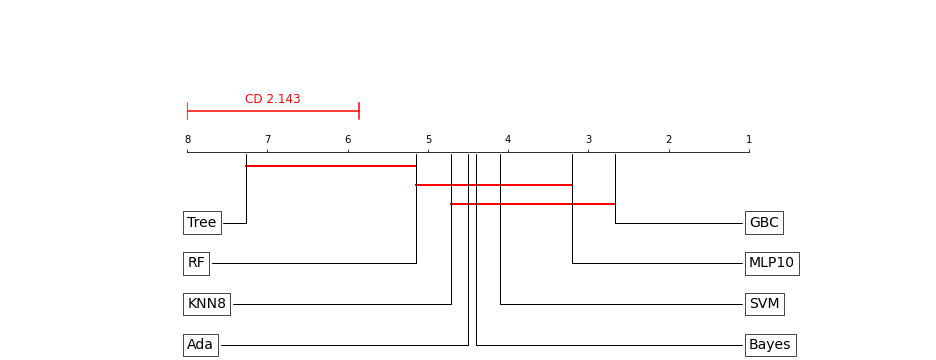
\includegraphics[width=0.95\linewidth]{img/Nemenyi1.png}
\caption{Nemenyi CD diagram}
\label{fig:NemenyiCD}
\end{figure}
\end{document}
